\documentclass[a4paper]{article}
\usepackage[pdftex]{graphicx}
\usepackage[utf8]{inputenc}
\usepackage{enumerate}
\usepackage{amssymb}
\usepackage{icomma}
\usepackage{siunitx}
\sisetup{locale=DE}
\usepackage{tikz}
\usepackage{href-ul}
\hypersetup{
	colorlinks=true,
	linkcolor=blue,
	urlcolor=blue}
\usepackage{geometry}
\geometry{a4paper, top=15mm, left=15mm, right=15mm, bottom=15mm,
	headsep=10mm, footskip=12mm}

\begin{document}
	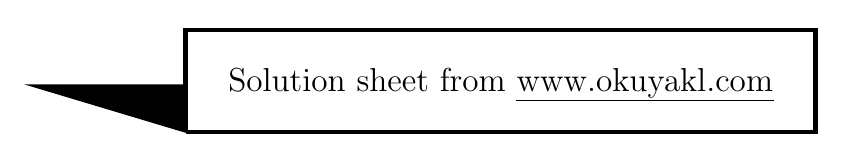
\begin{tikzpicture}(10,3)
		\draw[ultra thick](2,0) --(10,0) -- (10,1.3) --(2,1.3) -- (2,0);
		\draw[fill=black](2,0)-- (0,.6) -- (2,.6) -- (2,0);
		\node at (6,.6) {\large Solution sheet from \href{http://www.okuyakl.com}{www.okuyakl.com}};
	\end{tikzpicture}
	\vspace{0.5 cm}
	
	
	\noindent{\bf Task 1. a)}\\
	$$V= \SI{8,0}{\centi\meter^3}$$
	\vspace{0.5 cm}
	
	\noindent{\bf Task 1. b)}\\
	$$ F_1 = m\cdot g = \varrho_{Cu}\cdot V \cdot g = \SI{0.70}{\newton} $$
	\vspace{0.5 cm}
	
	\noindent{\bf Task 1. c)}\\
	$$ F_2 = \varrho_{Cu}\cdot V \cdot g - \varrho_{H_2O}\cdot V \cdot g = \SI{0.62}{\newton} $$
	\vspace{0.5 cm}
	
	\noindent{\bf Task 1. d)}\\
	It also shows the weight of the displaced liquid: Total $\SI{508}{\gram}$. The cube is still hanging on the dynamometer.
	\vspace{0.5 cm}
	
	\noindent{\bf Task 2. a)}\\
	The cup must be homogeneous, i.e. it must not have a base made of stone or similar.\\
	The measuring cylinder must be large enough so that the cup fits completely into it and can be submerged.\\
	The piece of silver must be large enough so that its volume and weight can be easily determined.
	\vspace{0.5 cm}
	
	\noindent{\bf Task 2. b)}\\
	\begin{itemize}
		\item The piece of silver and the cup are weighed on the scales and the respective weight $m_s, \quad m_p$ is noted.
		\item The measuring cylinder is filled with water up to a certain level.
		\item We completely immerse the cup in the measuring cylinder and note the increase in the level. $V_p$
		\item We take the cup out again, check the level, and dip the real silver chunk into it. We note $V_s$.
		\item We compare: $$ {m_s \over V_s} \stackrel{?}{=} \quad {m_p \over V_p} $$ If the density is the same, then the cup is real silver.
	\end{itemize}
	
	\vspace{0.5 cm}
	
	\noindent{\bf Task 3. a)}\\
	The difference in densities is:
	$$\Delta\varrho={1\over 4}\cdot \SI{1,3}{\kilogram\over{\meter^3}}= \SI{0.33}{\kilogram\over{\meter^3}} $$
	The payload is then:
	$$m=\Delta\varrho\cdot V = \SI{0.325}{\kilogram\over{\meter^3}} \cdot \SI{5000}{\meter^3}=\SI{1625}{\kilogram} \approx\SI{1.6}{\tonne}$$
	\vspace{0.5 cm}
	
	\noindent{\bf Task 3. b)}\\
	The difference in densities is:
	$$\Delta\varrho= \SI{1,3}{\kilogram\over{\meter^3}}-\SI{0.178}{\kilogram\over{\meter^3}} = \SI{1,1}{\ kilogram\over{\meter^3}} $$
	The volume is then:
	$$ V= {m \over \Delta\varrho}={\SI{1625}{\kilogram}\over \SI{1,122}{\kilogram\over {\meter^3}}}=\SI{1448}{\ meter^3}\approx\SI{1,4e3}{\meter^3}$$
	\vspace{0.5 cm}
	
	\noindent{\bf Task 4.}\\
	The density of the stone is ${9\over 10}$ of the density of the liquid, so
	$$\varrho_{Stein}=0.9\cdot \SI{3,1}{\gram\over\centi{\meter^3}}=\SI{2.8}{\gram\over\centi{\meter^3}}$$
	The volume of the stone is therefore:
	$$V_{Stein}={m \over \varrho_{Stein}}={\SI{80}{\gram}\over \SI{2.79}{\gram\over\centi{\meter^3}}} =\SI{28.7}{\centi {\meter^3}}\approx \SI{29}{\centi \meter^3}$$
	\vspace{0.5 cm}
	
	\noindent{\bf Task 5.}\\
	The formula for gravity pressure is:
	$$p=g\cdot \varrho \cdot h =\SI{9,81}{\meter\over {\second^2}} \cdot \SI{1000}{\kilogram\over {\meter^3}}\cdot h = \SI{7}{\kilo\pascal}$$
	\vspace{0.5 cm}
	
	\noindent{\bf Task 6.}\\
	\renewcommand{\arraystretch}{2}
	\begin{tabular}{|p{1.2 cm}|p{1.7 cm}|p{1.7 cm}|p{1.7 cm}|p{1.7 cm}|p{1.7 cm}|p{1.7 cm}|p{1.7 cm}|}
		\hline
		& non-swimmer pool & diving pool & North Sea & Lake Constance & Lake Baikal & Atlantic Ocean & Mariana Trench \\
		\hline
		Depth h &$\SI{1.20}{\meter}$ &$\SI{4.8}{\meter}$ &$\SI{50}{\meter}$ &$\SI{250}{ \meter}$ &$\SI{1642}{\meter}$ &$\SI{3500}{\meter}$ &$\SI{11}{\kilo\meter}$ \\
		\hline
		Pressure &$\SI{12}{\kilo\pascal}$ &$\SI{48}{\kilo\pascal}$ &$\SI{0.5}{\mega\pascal}$ &$\SI{ 2.5}{\mega\pascal}$ & $\SI{16}{\mega\pascal}$ &$\SI{35}{\mega\pascal}$ & $\SI{110}{\mega\ pascal}$\\
		\hline
	\end{tabular}
	
	\begin{center}
		\includegraphics[width=7 cm]{../../viecher/eendcomic.pdf}
		
		Here you can go back to the \href{https://www.okuyakl.de/phys/p9achL078/ae078.pdf}{task sheet}
	\end{center}
	
\end{document}